\begin{figure}[!h]
	\centering
	\subfigure[\simulink shema za hitrostne vodenje]
	{
		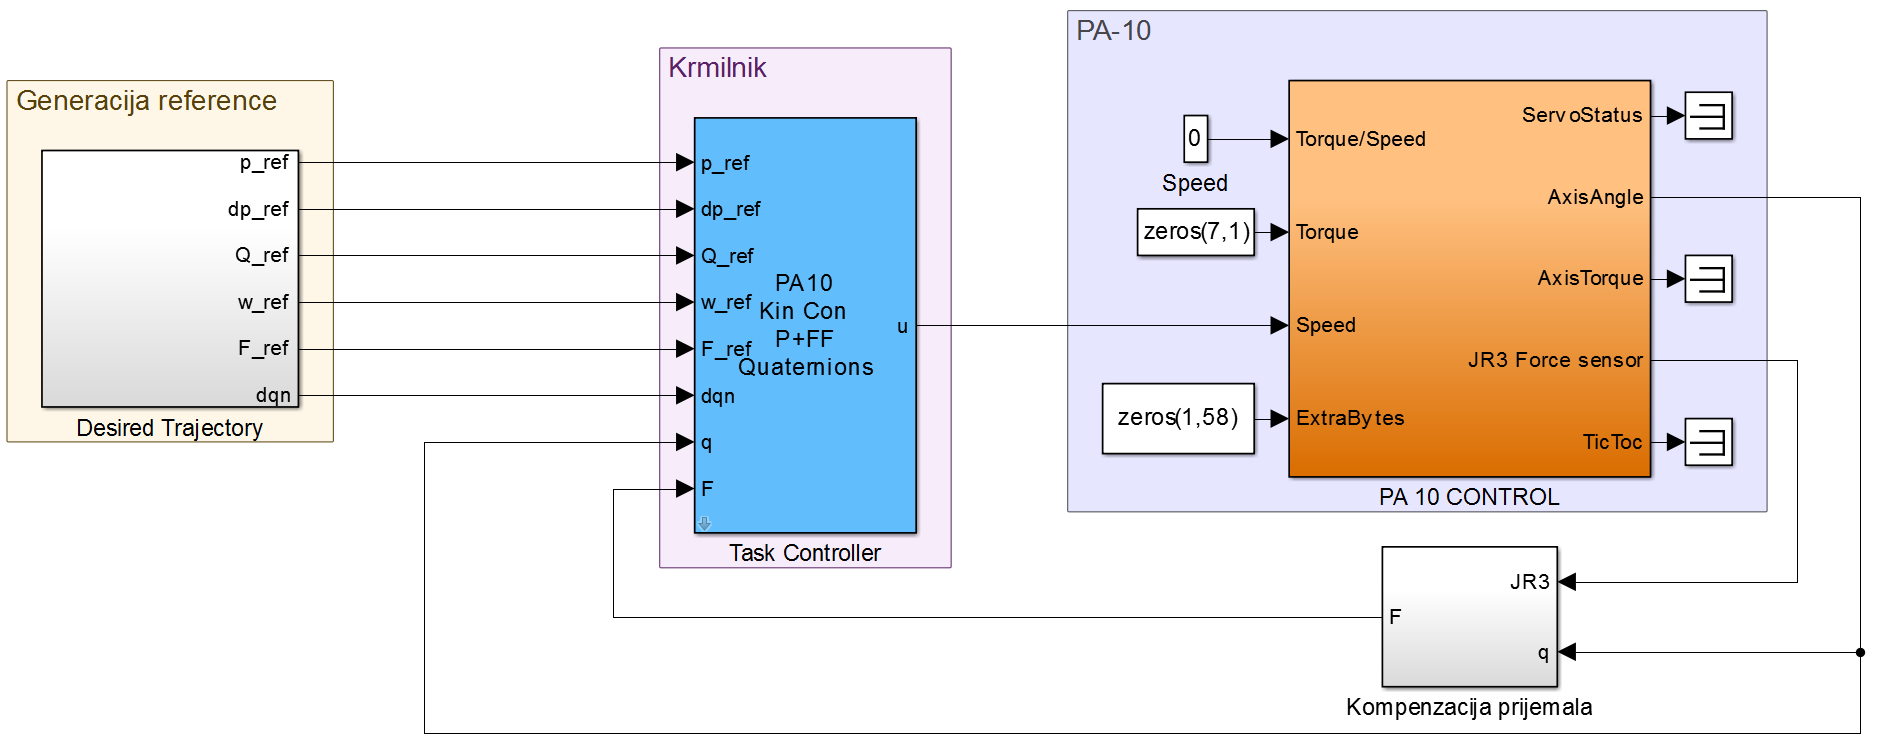
\includegraphics[trim={0 0cm 0 0cm},scale=0.2]{./Slike/velocity_control.png}
	}
	\subfigure[\simulink shema za navorno vodenje]
	{
		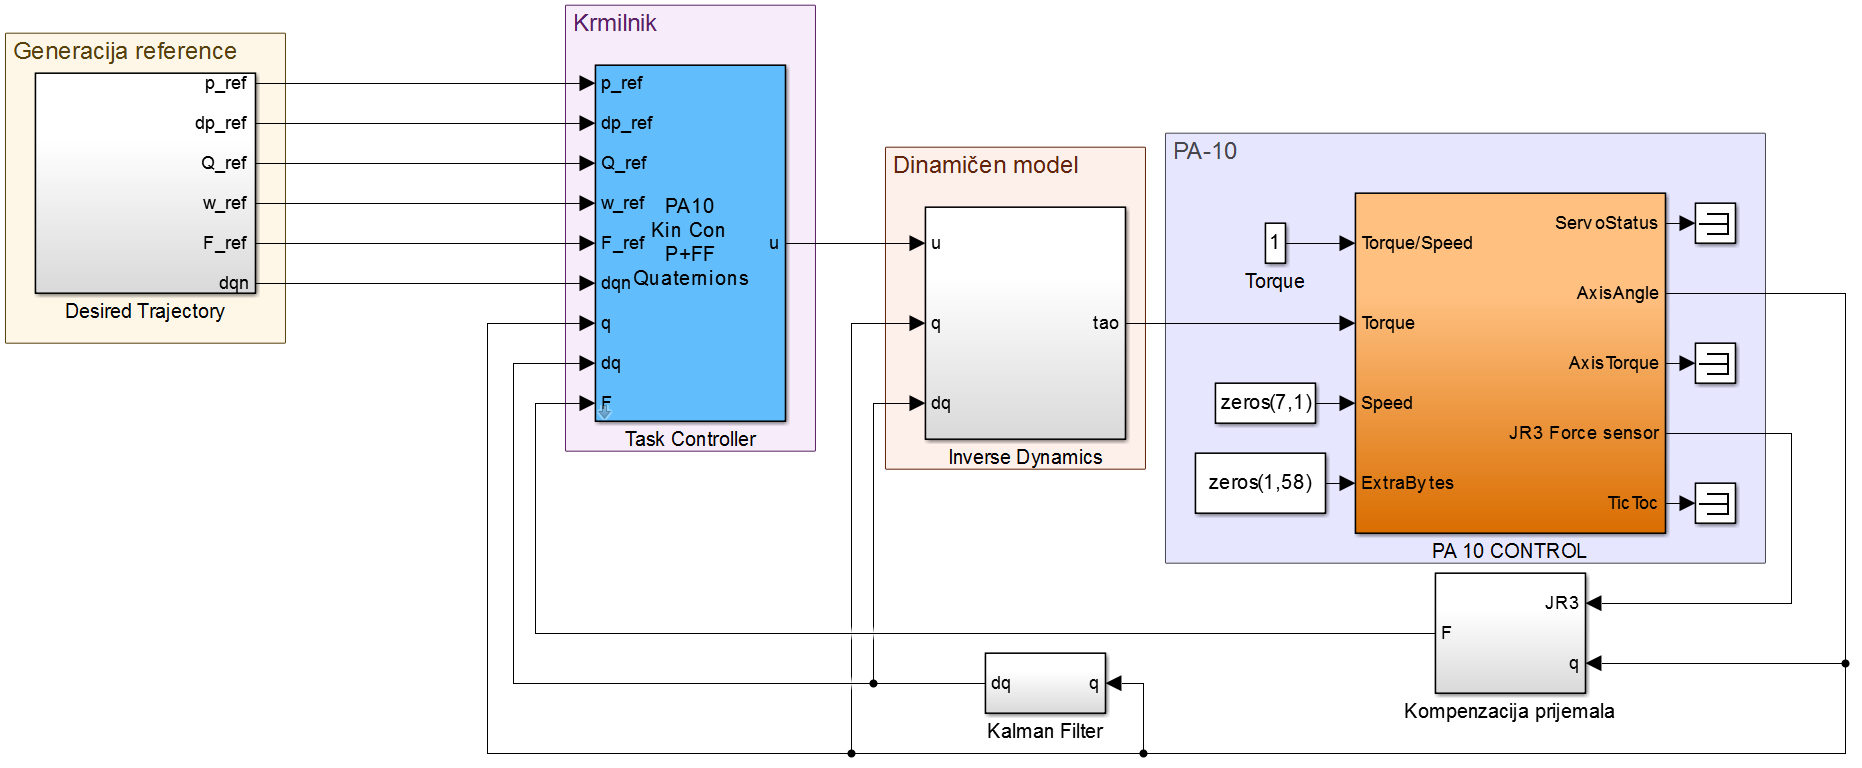
\includegraphics[trim={0 0cm 0 0cm},scale=0.2]{./Slike/torque_control.png}
	}
	\caption{\simulink shemi za vodenje robota PA-10 po prostoru naloge.}
	\label{fig:simulink_vel_tq_control}
\end{figure}
